\section*{Results}
\subsection*{ERP Analysis}
%As proposed in \cite{schaefer_name_2011}, we computed grand average \acp{ERP} by aggregating over all trials (excluding the cue clicks) of the same stimulus from all subjects except P05 (due to the movement artifacts).
Schaefer \etal \cite{schaefer_name_2011} used very short stimuli (3.26s) allowing each stimulus to be repeated many times during during the experiment. 
This allowed them to average across hundreds of short trials. 
They then concatenated the grand average ERPs and applied a \ac{PCA}, which resulted in clearly defined spatial features. The time courses of these spatial features allowed for classification of their stimuli. We started by trying to replicate these results. 
We had fewer repetitions of our stimuli. Therefore, to preserve as much data as possible we used the full length of the trials as opposed to the first 3.26 seconds. We computed grand average \acp{ERP}s by aggregating over the full length of all trials (excluding the cue) of the same stimulus from all subjects. We then concatenated the grand average \acp{ERP} and applied a \ac{PCA}. This resulted in principle components with poorly defined spatial components \autoref{fig:components} (A and B).

In order to preserve even more of the data and we took an alternative approach and performed a \ac{PCA} on the concatenated raw trials without first calculating an average across trials. This produced clearly defined spatial components \autoref{fig:components} (C and D). Except for their (arbitrary) polarity the components are very similar across the two conditions, which replicates the results found in \cite{schaefer_name_2011}.

\begin{figure}[t] 
  \begin{center}
    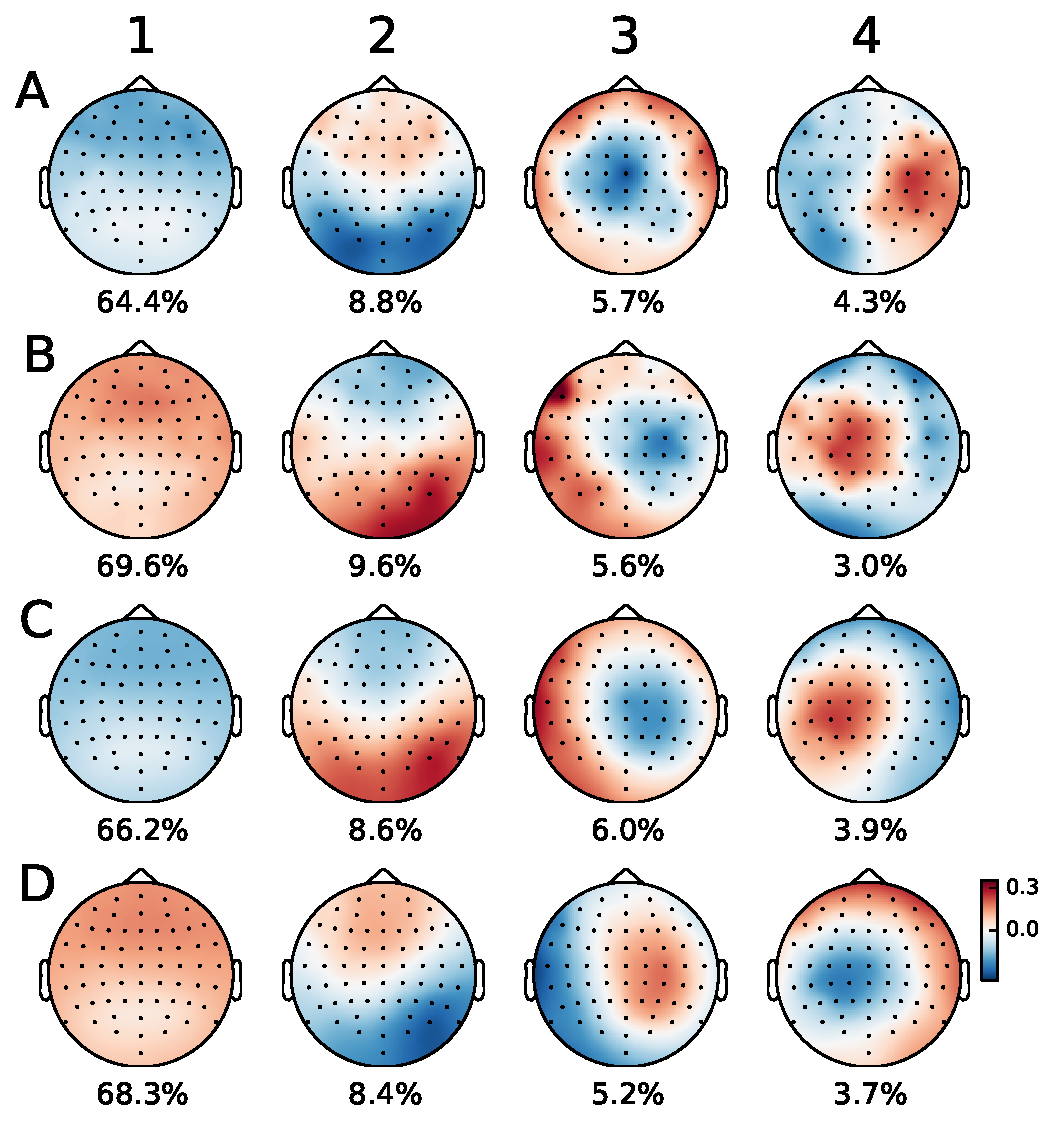
\includegraphics[width=0.8\textwidth,keepaspectratio=true]{Figures/principle_components.pdf}
%   \\\vspace{-0.8em}
    \caption{%
Topographic visualization of the top 4 principle components with percentage of the explained signal variance. %.\newline
Channel positions in the 64-channel EEG layout are shown as dots.
Colors are interpolated based on the channel weights.
%\hl{Polarity has no specific semantic.}
The PCA was computed on
\textbf{A}: the grand average \acp{ERP} of all perception trials,
\textbf{B}: the grand average \acp{ERP} of all cued imagination trials,
\textbf{C}: the concatenated perception trials,
\textbf{D}: the concatenated cued imagination trials.
}
    \label{fig:components}
  \end{center}
% \vspace{-2em}
\end{figure}

\subsection*{Component Waveform Correlations}
Table of values.
To show how similar.
Component waveforms ? correlation between perception and imagination 

\subsection*{Classification}
Schaefer \etal \cite{schaefer_name_2011} were able to use the unique time course of the component responsible for the most variance to differentiate between stimuli.
Analyzing our components we have not yet been able to reproduce this significant stimulus classification accuracy. 
This could be caused by our much smaller number of trials which are substantially longer than those used by \cite{schaefer_name_2011}. 
\hl{do we have numbers we can show here?}

Different classification approach ? convolutional auto encoder (CAE) to produce components. What are the parameters?
Fed waveforms of these components to convolutional neural network (CNN). What are the parameters here? 2 experiments ? 12 class and 2 class